%!TEX encoding = UTF-8 Unicode  
\documentclass{article}  
\usepackage{xeCJK}
\setCJKmainfont[BoldFont=STZhongsong, ItalicFont=STKaiti]{STSong}
\setCJKsansfont[BoldFont=STHeiti]{STXihei}
\setCJKmonofont{STFangsong}
\usepackage{graphicx}
\usepackage{amsmath}
 \usepackage{clrscode}
\usepackage{listings}
\usepackage{enumerate}
\lstset{language=C++}%这条命令可以让LaTeX排版时将C++键字突出显示

\lstset{breaklines}%这条命令可以让LaTeX自动将长的代码行换行排版

\lstset{extendedchars=false}%这一条命令可以解决代码跨页时,章节标题,页眉等汉字不显示的问题




\begin{document}  

\title{开题报告}
\date{}

\maketitle


\textbf{一、问题提出的背景}
      \qquad
\newline
    
     \textbf{1、背景介绍}
     \qquad
      近年来,在工程应用中,求解高阶矩阵的需求日益增长,全矩阵运算脱离了实际的硬件限制,为了满足这一日益增长的需求,同时这些矩阵通常都有着一个特征——非零元远少于零元,稀疏矩阵这门学科便应运而生。
在 20 世纪 60 年代研发电子网络的电子工程师们是最早的去利用稀疏性来应用稀疏矩阵进行工程上的计算的。[1]
而在微分方程数值解、线性规划等的有限元分析中,经常出现求解高阶稀疏线性方程组,如利用全矩阵进行存储,则需要$n^2$的空间复杂度和$n^3$的乘法运算时间复杂度,显然,这种程度的运算量是无法被微型计算机,甚至是工作站所接受的。
而利用矩阵的稀疏性,可以有效地减小消耗很多无谓的存储空间以及无谓的计算,在很大的程度上降低了时间和空间复杂度,降低了计算对硬件的需求,使计算成为可能。
\newline

 \textbf{2、本研究的意义和目的}
 \newline
 在实际工程计算中,尤其是在微分方程数值解、线性规划等的有限元分析中,经常出现高阶的矩阵运算,经常出现百万阶、千万阶的矩阵运算,而如果使用全矩阵运算,假设是百万阶的float类型的矩阵,则需要$4*10^{12}B$来存储,也就是4TB的空间,这显然是无法被微型计算机甚至是工作站所接受的。但是通常这些矩阵具有稀疏的性质,拥有着大量的零元,而且通常阶数越高稀疏度越高。这就可以在相当大的程度上减少了存储对于硬件的压力。同时,在计算中,大量对于0的运算是五位的消耗资源的操作,也可以利用稀疏矩阵来避免这些无谓的操作。而在本研究中编写的稀疏矩阵库可以用来方便快捷的实现稀疏矩阵的存储以及一些基本运算,避免了使用者大量编写存储底层的代码,提高开发效率。\newline
 
\textbf{3、研究现状}\newline
在稀疏矩阵这些年的发展中,出现了很多的存储方法,比如:对角线存贮法、对称矩阵的变带宽存贮法、坐标存贮法、Elipack-Itpack存贮法、CSR存贮法、Shermans存贮法、超矩阵存贮法、动态存贮方案等。\newline
如行压缩存储方式(Compressed Row Storage):
CRS存储可以高效地存取任意一行非零元素,但存取任意一列非零元则需要遍历整个CRS存储结构。相应地,与CRS存储的稀疏矩阵相关的算法要高效的编程实现,算法的计算顺序必须按行来进行。[1]
下面对应于CRS存储:
\newline\newline\newline\newline\newline\newline\newline\newline

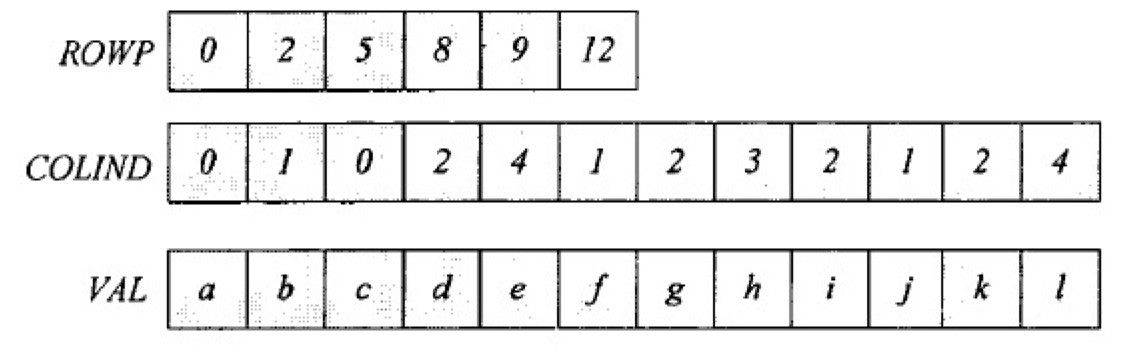
\includegraphics[scale=0.25]{crs.png} \newline
我们可以发现,ROWP数组存储的时行非零元的增长量。COLIND则存储的是列索引值,典型的C语言结构实现为\newline
\begin{lstlisting}

struct cr_matrix{ 
	int *Ri;/*col index*/ 
	int *Rp;/*length nrow+1*/ 
	double *Rx; 
	int Rncol;
	int Rnrow;
};

\end{lstlisting}
在早期计算机时,串行的算法占到主流,自然,稀疏矩阵的存储方式以及稀疏矩阵的计算都是为了串行算法服务的。但是随着计算机的发展,计算机集群、多核CPU、GPU并行等的出现,让并行算法在计算时间上远远地超越了串行算法,为了更好的适应并行计算中的稀疏矩阵计算,出现了许多新的算法以及存储方式。例如对于非结构化的矩阵,基于CUDA框架下的SCOO形式的SpMV算法比利用基于Cusp库的SCOO具有更高的效率。[2]
\newline

而在做稀疏矩阵的计算时,通常都是做一系列的基本运算,如:矩阵转置、矩阵向量乘法、矩阵矩阵乘法、数乘等。为了能得到更好的效率,许多研究者致力于寻找对于这些计算最优的存储结构及计算算法,同时提供了许多类库供科学计算使用,如:Portable, ExtensibleToolkit for Scientific Computation(PETSc)、Boost、GNU Scientific Library (GSL)等。\newline
例如,在Boost-uBLAS中有着稀疏矩阵的模板mapped\_matrix<T, F, A>(元素映射矩阵存储形式)、compressed\_matrix<T, F, IB, IA, TA>(压缩存储格式)、coordinat\_matrix<T, F, IB, IA, TA>(坐标存储格式)。
分别有着如下示例:[3]\newline
\textbf{mapped\_matrix:}
\begin{lstlisting}

#include <boost/numeric/ublas/matrix_sparse.hpp>
#include <boost/numeric/ublas/io.hpp>

int main () {
    using namespace boost::numeric::ublas;
    mapped_matrix<double> m (3, 3, 3 * 3);
    for (unsigned i = 0; i < m.size1 (); ++ i)
        for (unsigned j = 0; j < m.size2 (); ++ j)
            m (i, j) = 3 * i + j;
    std::cout << m << std::endl;
}

\end{lstlisting}

\textbf{compressed\_matrix:}
\begin{lstlisting}

#include <boost/numeric/ublas/matrix_sparse.hpp>
#include <boost/numeric/ublas/io.hpp>

int main () {
    using namespace boost::numeric::ublas;
    compressed_matrix<double> m (3, 3, 3 * 3);
    for (unsigned i = 0; i < m.size1 (); ++ i)
        for (unsigned j = 0; j < m.size2 (); ++ j)
            m (i, j) = 3 * i + j;
    std::cout << m << std::endl;
}

\end{lstlisting}

\textbf{coordinate\_matrix:}
\begin{lstlisting}

#include <boost/numeric/ublas/matrix_sparse.hpp>
#include <boost/numeric/ublas/io.hpp>

int main () {
    using namespace boost::numeric::ublas;
    coordinate_matrix<double> m (3, 3, 3 * 3);
    for (unsigned i = 0; i < m.size1 (); ++ i)
        for (unsigned j = 0; j < m.size2 (); ++ j)
            m (i, j) = 3 * i + j;
    std::cout << m << std::endl;
}
\end{lstlisting}


在多年的研究中,各种相关的研究成果页层出不穷,例如,
根据Michele Martone的研究成果,在对称矩阵乘法,或者转置的矩阵向量乘法中,RSB格式的迭代算法效率是比较高的[4]。
而在李佳佳,张秀霞,谭光明,陈明宇的研究中,得到了影响矩阵性能的参数集,可以利用该参数集提取矩阵特征,并输出最优存储格式,供数值解法器和上层应用调用。[5]
为了适用于大数据集计算以及克服现有稀疏矩阵乘法算法低效的问题,郑建华,朱 蓉,沈玉利提出了一种基于向量线性组合(VLC)的矩阵乘法处理模式,同时采用MapReduce计算模型实现了基于VLC模式的并行矩阵乘法算法。[6]
而在集群计算方面,负载平衡是不能不提到的,为了更好地发挥集群计算的计算能力,付朝江博士给出了基于贪婪分配的稀疏矩阵与向量乘的负载平衡的解决方案。[7]
\newline


\textbf{二、论文的主要内容和技术路线}
      \qquad
\newline

     \textbf{1、主要研究内容} \qquad
\newline
     
     在linux平台下,基于g++编译器,编写稀疏矩阵存储的C++库,实现稀疏矩阵的行压缩存储方式(Compressed Row Storage),同时实现一些稀疏矩阵的基本运算,如矩阵乘法、数乘等,实现多线程计算。
\newline

     \textbf{2、技术路线} \qquad
\newline
实现稀疏矩阵的行压缩存储方式(Compressed Row Storage),利用C++的STL中的vector来存储数据。
\newline
     利用thread库实现多线程并行计算,更为有效地利用CPU的并行性能。利用mutex互斥锁保障进程安全性,防止出现“脏”数据。
\newline
	

     \textbf{3、可行性分析}
     \begin{enumerate}[1]
\item 	linux平台较Windows更为稳定,不容易出现宕机,且被工程界广为使用
\item 	g++是GNU的C++编译器,历史悠久,经历过多年考验,有着成熟的文档和社区帮助
\item		稀疏矩阵这门学科已存在多年,存在着成熟的存储方案及相关算法
\item		多线程的锁机制已出现多年,可以有效地保障进程安全性
\item		基于标准C++开发,有着良好的跨平台性

\end{enumerate}


\textbf{三、研究计划进度安排及预期目标}
      \qquad
\newline
 

     \textbf{1、进度安排}\qquad \newline
     2014年11月24日-2014年12月21日,文献收集整理,基础知识学习。\newline
2014年12月22日-2015年1月4日,讨论算法模型,确定方案和技术路线。\newline
2015年1月5日-2015年1月29日,完成文献综述、开题报告和文献资料翻译。\newline
2015年3月9日-2015年4月5日,程序编写、调试。\newline
2015年4月6日-2015年5月3日,数值实验和数据收集。\newline
2015年5月4日-2015年5月31日,毕业论文撰写。\newline
2015年6月1日-2015年6月14日,ppt制作,准备答辩。
\newline



     \textbf{2、预期目标}
     利用c++在g++编译器linux平台下实现稀疏矩阵的行压缩存储方式(Compressed Row Storage)存储。可以并行计算稀疏矩阵的矩阵乘法、数乘等运算。
\newline
 
 \textbf{四、参考文献}
      \qquad
\newline
  [1]张永杰、孙秦.稀疏矩阵存储技术[J].长春理工大学学报,2006年,03期:38-41.\newline
      [2]Hoang-Vu Dang,  Bertil Schmidt.CUDA-enabled Sparse Matrix–Vector Multiplication on GPUs
using atomic operations[J].Parallel Computing, 2013,Vol.39 (11):737-750.\newline
  [3]Joerg Walter and Mathias Koch.Boost 1.57.0 Library Documentation-uBLAS. http://www.boost.org/doc/libs/1\_57\_0/libs/numeric/ublas/doc/index.html, 2011\newline
  [4]Michele Martone.Efficient multithreaded untransposed, transposed or symmetric sparse matrix–vector multiplication with the Recursive Sparse Blocks format[J].Parallel Computing, 2014,40:47-58.\newline
  [5]李佳佳,张秀霞,谭光明,陈明宇.选择稀疏矩阵乘法最优存储格式的研究[J].计算机研究与发展 , Journal of Computer Research and Developmen,2014年,04期:882-894.\newline
  [6]郑建华,朱 蓉,沈玉利.Sparse matrix multiplication algorithm based on MapReduce[J].仲恺农业工程学院学报,2013年,03期:45-50.\newline
[7]付朝江.基于贪婪分配的稀疏矩阵与向量乘的负载平衡[J].福建工程学院学报 ,2010年,01期:79-82.\newline
\end{document}  
